\documentclass[12pt]{article}

\usepackage{amsmath}
\usepackage{graphicx}
\usepackage{float}
\graphicspath{{figures/}}

\title{Glutamate GPCR, IP3 and Calcium Dynamics}

\begin{document}

\date{July 22, 2020}
\maketitle

\tableofcontents

\pagebreak
%%%%%%%%%%%%%%%%%%%%%%


\section{Previous Calcium Dynamics Model}

In previous work, Greg and Marsa have constructed a model for astrocyte calcium dynamics given IP3 as an input to the system, described by $p(t)$ as a function of time \cite{taheri2017diversity, handy2017mathematical}. Their model was based on pieces from various other papers, and tweaks to parameters ($v_{IP3R}$, $v_{leak}$, $v_{PMCA}$, $k_{out}$, $k_{PMCA}$, $k_{SOC}$, $\delta$, $a_2$) were made such that the model responded to a double-exponential IP3 pulse in a reasonable way. In particular, the dynamics of the model were matched to a single peak response of a real astrocyte by tweaking these parameters (see Fig \ref{fig:calcium_model_parameter_tweaking}). 

\begin{figure}[H]
	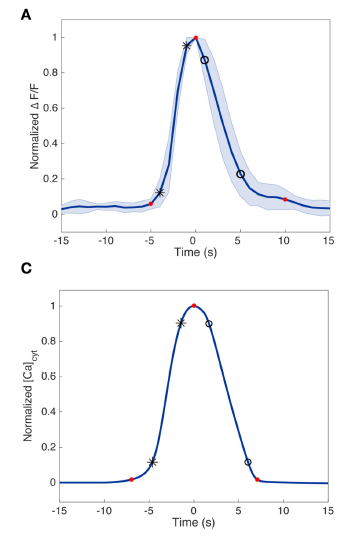
\includegraphics[width=0.5\linewidth]{taheri_fig3_clip.png}
	\centering
	\caption{Clip from Figure 3 of \cite{taheri2017diversity} showing how the model is fit to a real calcium trace, assuming we have a reasonable IP3 transient as an input to the system.}
	\label{fig:calcium_model_parameter_tweaking}
\end{figure}

\subsection{Oscillating Behavior}

Given a bath application of IP3, the calcium model will begin to oscillate. This is explored both through numerical simulation and through observation of the bifurcation diagram, with IP3 as a control parameter (see Fig \ref{fig:calcium_model_oscillations}).

\begin{figure}[H]
	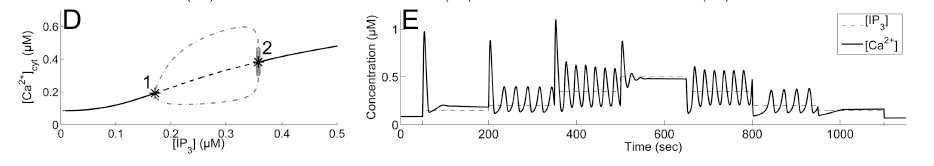
\includegraphics[width=1\linewidth]{handy_fig3_clip.png}
	\centering
	\caption{Clip from Figure 3 of \cite{handy2017mathematical} showing (D) the bifurcation diagram of the calcium dynamics model with IP3 as a control parameters; (E) stepwise IP3 inputs demonstrate calcium oscillations at different levels of IP3}
	\label{fig:calcium_model_oscillations}
\end{figure}


%%%%%

\subsection{Classifying Calcium Responses}

Given applications of IP3 that last for a shorter total amount of time, the system may have a few oscillations before the input is cut off and the calcium returns to baseline levels. Thus given different IP3 inputs, we can observe different types of calcium dynamics. In \cite{taheri2017diversity}, the types of calcium responses are labeled as single peak (SP), multi peak (MP), plateau (PL), or long lasting (LL) responses. Examples of this are given in \ref{fig:calcium_response_types}.

\begin{figure}[H]
	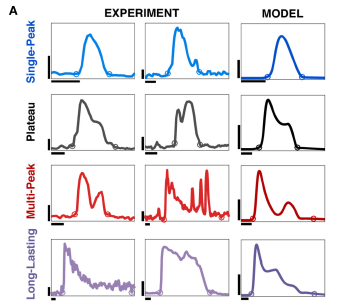
\includegraphics[width=0.5\linewidth]{taheri_fig2_clip.png}
	\centering
	\caption{Clip from Figure 2 of \cite{taheri2017diversity} showing experimentally and numerically derived calcium traces of each of the 4 types of calcium response (SP, MP, PL, LL).}
	\label{fig:calcium_response_types}
\end{figure}

The IP3 inputs are given by a double exponential, which are uniquely defined by their 4 parameters, $d_{rise}$, $d_{decay}$, $r_{rise}$, $r_{decay}$. IP3 inputs were created by taking a range of each of these parameters. They were fed into the calcium dynamics model and using a classification algorithm, Marsa and Greg determined how often certain types of response appeared (see Fig \ref{fig:calcium_response_frequency_scatter}). 

\begin{figure}[H]
	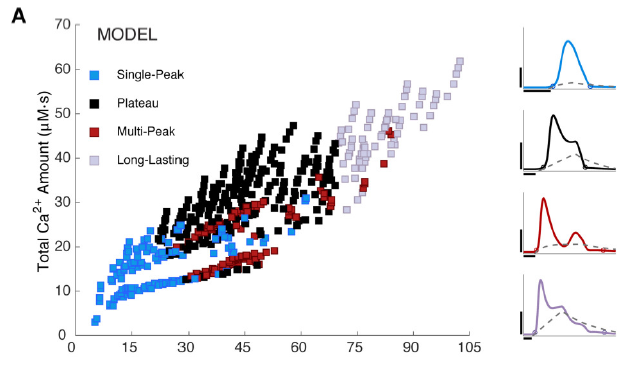
\includegraphics[width=0.5\linewidth]{taheri_fig4_clip.png}
	\centering
	\caption{Clip from Figure 4 of \cite{taheri2017diversity} showing the types of calcium responses that were recorded for various IP3 inputs. Here, the x-axis shows the total duration of the calcium response.}
	\label{fig:calcium_response_frequency_scatter}
\end{figure}

Marsa noted that the frequency of type of calcium response varied depending on the part of astrocyte that was being recorded (soma, large processes, or small processes). Then, matching these classification frequencies against the classification frequencies given by certain ranges of IP3 input parameter, they determined the differences in IP3 transients that would need to be generated for each of these astrocytic regions.




%%%%%%%%%%%%%%%%%%%%%%%%%%%%%%%%%%%%%%%

%%%%%%%%%%%%%%%%%%%%%%%%%%%%%%%%%%%%%%%




\section{IP3 Dynamics}

The first thing we have added on to the calcium dynamics model is a model for IP3 dynamics. The ODE for IP3 is

\begin{equation}
\frac{dp}{dt} = IP3_{prod} - IP3_{deg}
\end{equation}
\begin{align*}
IP3_{prod} &= v_{\beta} G^* + v_\delta \frac{k_\delta}{1+p} \frac{c^2}{c^2 + k^2_{PLC\delta}}\\
IP3_{deg} &= r_{5p}p + v_{3k} \frac{c^4}{c^4 + k^4_d} \frac{p}{p + k_3} \ ,
\end{align*}
where $G^*$ is the new control parameter (replacing IP3 from the calcium-only model) which represents the activity of an upstream glutamate G-protein coupled receptor (GPCR). 

Fig \ref{fig:gstar_steps} shows the dynamics of this new system with IP3 as a variable and $G^*$ as the control parameter, and Fig \ref{fig:c_gstar_bifurcation} shows the bifurcation diagram. These can be compared with Fig \ref{fig:calcium_model_oscillations}. The system largely has the same shape of bifurcation diagram, and qualitatively similar solutions can be achieved with a stepping input, just as with the previous system using IP3 as the control parameter.

When adding the IP3 dynamics, the equilibrium state of the system with no input changed. To keep the equilibrium state close to that of the original system, I modified the value of $r_{5p}$, which is the degradation rate of IP3, from $0.08$ to $0.118$. 

\begin{figure}[H]
	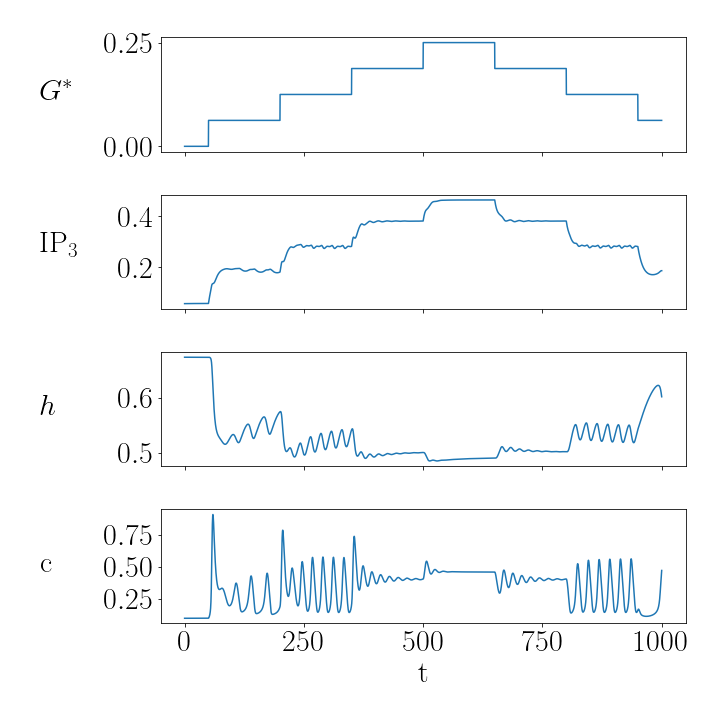
\includegraphics[width=0.7\linewidth]{Gstar_steps.png}
	\centering
	\caption{Solutions to the ODE system with $G^*$ as the control parameter, increasing and decreasing in discrete steps. This shows some of the range of oscillatory behaviors that the system can undergo.}
	\label{fig:gstar_steps}
\end{figure}

\begin{figure}[H]
	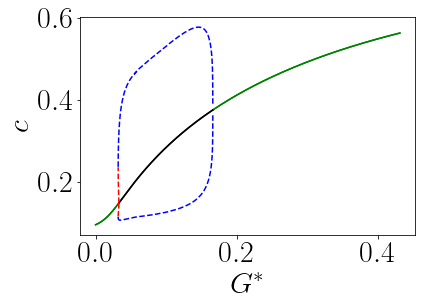
\includegraphics[width=0.5\linewidth]{c_Gstar_bifurcation.png}
	\centering
	\caption{Bifurcation diagram of the ODE system with $G^*$ as the control parameter.}
	\label{fig:c_gstar_bifurcation}
\end{figure}



%%%%%%%%%%%%%%%%%%%%%%%%%%%



\subsection{Class I vs. Class II System}

When talking about astrocyte calcium dynamics models, generally they fall under one of two classes of model, depending on their assumption for how calcium or IP3 feedback can induce oscillations in the system. In the Class I model, the assumption is that calcium has feedback regulation on the IP3 receptor channel, a channel that allows calcium to flow from the ER to the cytoplasm when activated by IP3. In this model, IP3 is not required to oscillate in order to drive oscillations in cytosolic calcium levels.

In the Class II model, the assumption is that calcium has feedback on IP3 production or degradation (or on both), thus it causes oscillations in IP3, which in turn cause oscillations in cytosolic calcium \cite{han2017mathematical}.

It is slightly unclear to me whether the Class I/II assumptions refer specifically to how calcium oscillations are produced, or if they refer to the feedback action of calcium onto the dynamical system. In the latter case, it would seem to me that Class I/II are not incompatible.

Figure 1 from \cite{han2017mathematical} (reproduced here in Fig \ref{fig:calcium_ip3_spike_timing}) shows relative spike timings of calcium and IP3 in an experimental astrocyte. The order (calcium spiking before IP3) would suggest that oscillations in IP3 are driven by oscillations in calcium, and not the other way around, thus supporting the Class I assumption. Our dynamical model is also a Class I model, which is apparent from the fact that calcium oscillations are found even when IP3 is treated as a parameter. 

\begin{figure}[H]
	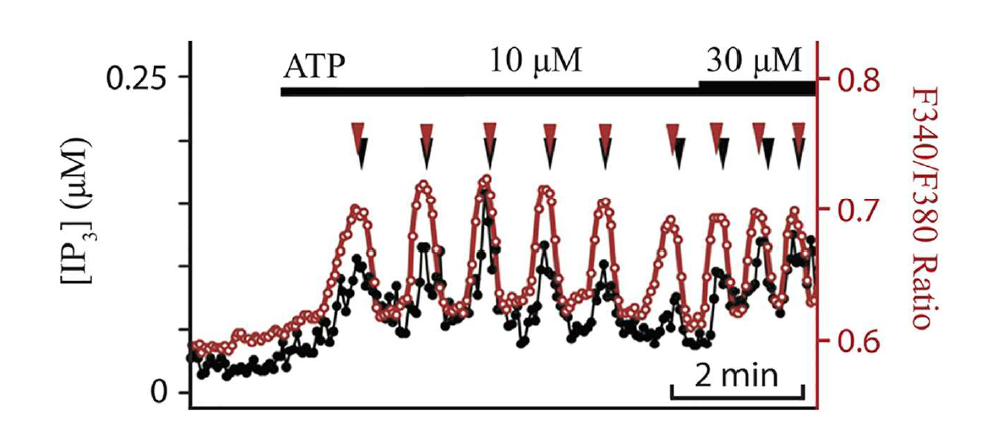
\includegraphics[width=0.8\linewidth]{calcium_ip3_spike_timing.png}
	\centering
	\caption{Figure 1 from \cite{han2017mathematical}. Shows relative spike timings for calcium (red) and IP3 (black) during experimental stimulus of astrocyte. }
	\label{fig:calcium_ip3_spike_timing}
\end{figure}



%%%%%%%%%%%%%%%%%%%%%%%%%%%%%%%%%%%



\subsection{Positive and Negative Feedback}

In the previous subsection, we discuss the differences between Class I and Class II calcium dynamics for astrocyte models. Although we do not require feedback from calcium onto IP3 to produce oscillations, we do include it in our model, both with positive and negative calcium to IP3 feedback (here, I should look for citations exploring the evidence for and against feedback, even treating the existence of positive and negative feedback separately). 

There are two important parameters for determining the strength of this feedback. Namely, $v_\delta$ controls the strength of positive feedback, while $v_{3k}$ controls the strength of negative feedback. See Section 2 for equations. Before I began working on this project, we had $v_\delta=2$, which produces oscillations that seem less physically realistic (see Fig \ref{fig:v3k_2_gstar_steps}). 

\begin{figure}[H]
	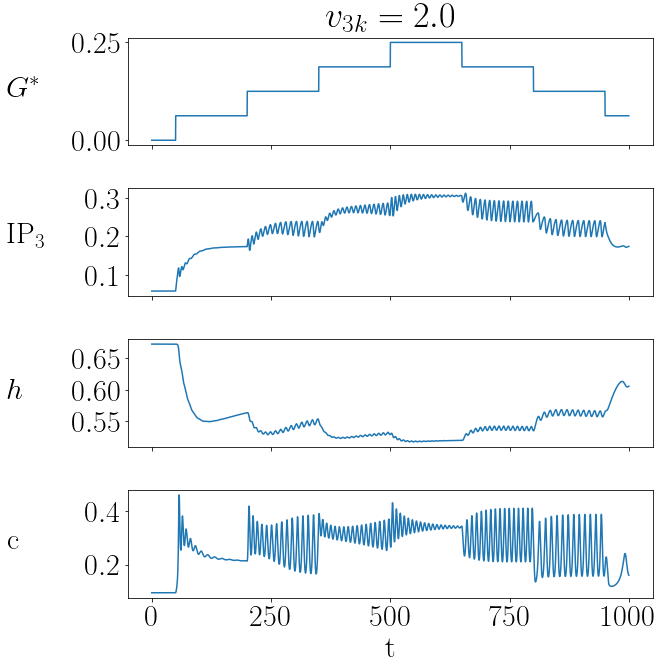
\includegraphics[width=0.7\linewidth]{v3k_2_Gstar_steps.png}
	\centering
	\caption{Solutions to the ODE system with $G^*$ as the control parameter, increasing and decreasing in discrete steps, with the parameter $v_{3k}=2$. Compare with Fig \ref{fig:gstar_steps}}
	\label{fig:v3k_2_gstar_steps}
\end{figure}

Marsa seems to suggest that such calcium to IP3 feedback has been found in some cells using this mechanism, such as in rat hepatocytes \cite{dupont2003ca2+}. She says that there is not conclusive evidence for astrocytes, but says that negative feedback seems less likely. \cite{dupont2003ca2+} also suggests that negative feedback is not necessary for oscillations (which is further evidence of a Class I system).

So what are the effects of positive and negative feedback? \cite{politi2006models} suggests that they have an impact on the frequency of calcium oscillation. We ran bifurcations with positive and negative feedback turned on, with one of them off, or with both off (see Fig \ref{fig:positive_negative_bifurcations}). In agreement with \cite{politi2006models}, we notice that positive feedback decreases the threshold of stimulation strength required to produce oscillations, which is apparent in the bifurcation diagrams (note that their system is a Class II system, but we still find agreement in this result). They also found that larger feedback increased the range of oscillation frequencies that can be exhibited by the calcium dynamics. We have yet to test whether this is true in our system as well.

\begin{figure}[H]
	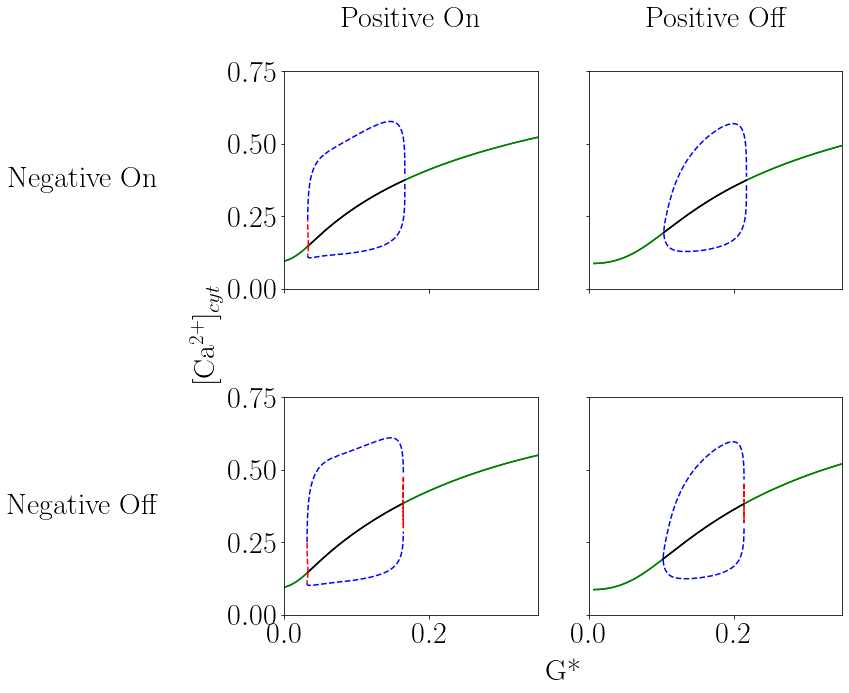
\includegraphics[width=0.7\linewidth]{positive_negative_bifurcations.png}
	\centering
	\caption{Bifurcation diagrams with $G^*$ as the control parameter with calcium to IP3 feedback turned on or off.}
	\label{fig:positive_negative_bifurcations}
\end{figure}

Although negative feedback does not seem to appreciably change the bifurcation diagram of the system, we did notice that it increased what seemed to be a delay period before the system begins oscillations.



%%%%%%%%%%%%%%%%%%%%%%%%%%%%%%%%%%%



\subsection{Oscillation Delays}

When the system is at equilibrium state with no input, and is then given a constant input of $G^*$ within its oscillatory range, its cytosolic calcium level first spikes, then begins oscillating (See Fig \ref{fig:varying_v3k_oscillation_delays}). We noticed that there is a slight delay between that initial spike and the time when the system enters stable oscillations, and that this length of time is increased as $v_{3k}$ is increased.

\begin{figure}[H]
	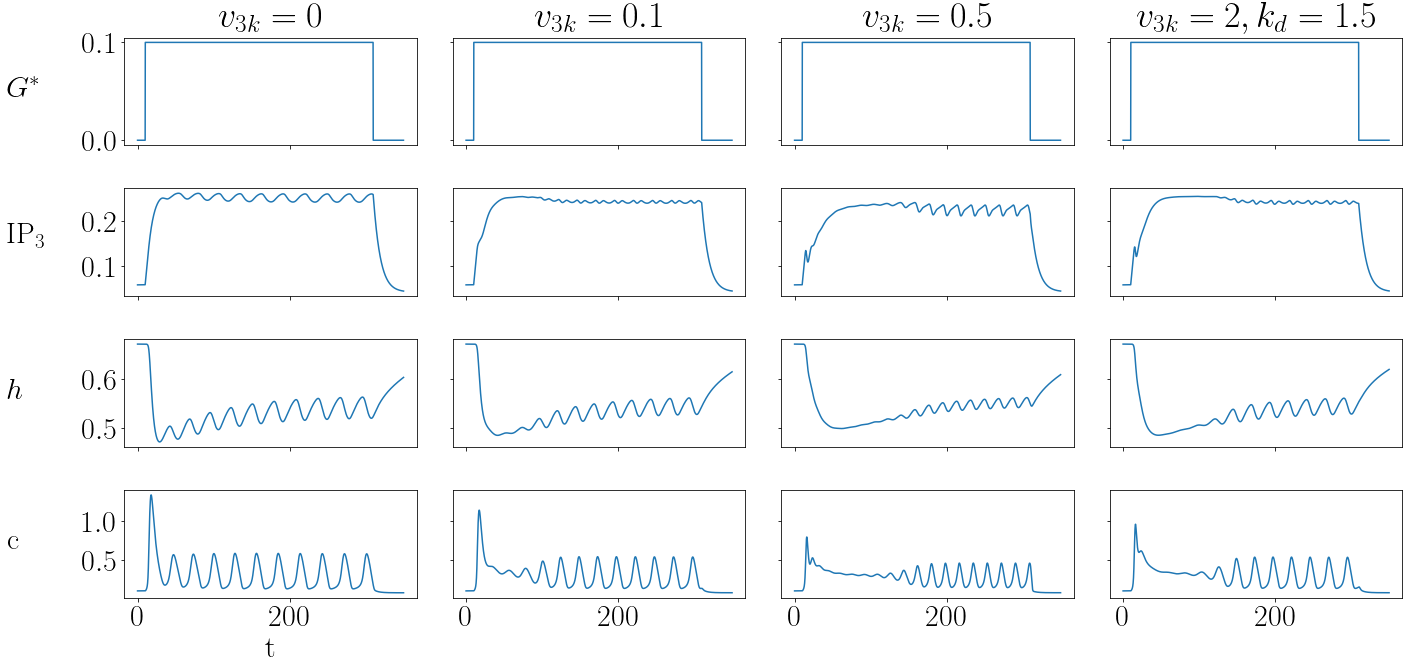
\includegraphics[width=1\linewidth]{varying_v3k_oscillation_delays.png}
	\centering
	\caption{Calcium and IP3 dynamics when given a constant input of $G^*=0.1$. As $v_{3k}$ is increased, there is an increasingly longer period of time between the initial spike and the time when the system has stable oscillations. }
	\label{fig:varying_v3k_oscillation_delays}
\end{figure}

We note that increases in $v_{3k}$ seem to also affect other qualities of the spiking behavior, such as amplitude and frequency. If $k_d$ (the half-max parameter of negative calcium to IP3 feedback) is increased as well as $v_{3k}$, some of the original character of the spiking with $v_{3k}$ small is returned. 


%%%%%%%%%


\subsubsection{Parameters that induce delays}

With the positive feedback fixed, we numerically solved the system for a range of $G^*$ and $v_{3k}$ (negative feedback strength) values. The results of this experiment are shown in Fig \ref{fig:oscillation_delay_times_v_delta_0.01}. In comparison, Fig \ref{fig:oscillation_delay_times_v_delta_0} shows this experiment with $v_\delta=0$ fixed. Although it is somewhat hard to tell from the coloring, when positive feedback is turned off, the delays occur less strongly towards the left Hopf bifurcation than when it is on. 

\begin{figure}[H]
	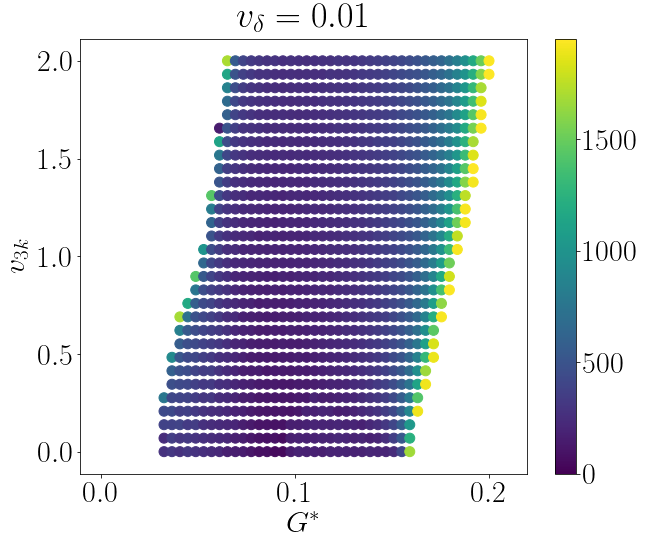
\includegraphics[width=0.6\linewidth]{oscillation_delay_times_v_delta_0_01.png}
	\centering
	\caption{Oscillation delay times with $v_\delta=0.01$ fixed and a range of $G^*$ and $v_{3k}$ values. Delay times here are calculated as the time it takes for the system to reach stable oscillations from $t=0$.}
	\label{fig:oscillation_delay_times_v_delta_0.01}
\end{figure}

\begin{figure}[H]
	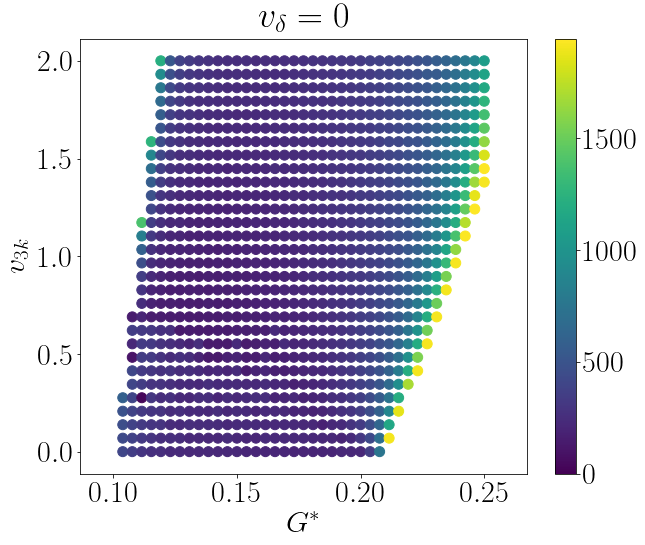
\includegraphics[width=0.6\linewidth]{oscillation_delay_times_v_delta_0.png}
	\centering
	\caption{Oscillation delay times with $v_\delta=0$ fixed and a range of $G^*$ and $v_{3k}$ values.}
	\label{fig:oscillation_delay_times_v_delta_0}
\end{figure} 

Delays are longest for higher values of $G^*$, especially at some critical value. This value seems like it should be the Hopf bifurcation point, however, it seems like the numerical solver I am currently using is not characterizing this correctly, as the bifurcation should be around $G^*=0.17$ for all values of $v_{3k}$ with $v_\delta=0.01$. XPP correctly has this critical value at the Hopf bifurcation. The overall trend shown in Fig \ref{fig:oscillation_delay_times_v_delta_0.01} is correct however.

Perhaps counter to our original assumptions, delays in reaching stable oscillations can occur when no positive or negative calcium to IP3 feedback is present. However, delays occur almost exclusively at the right Hopf bifurcation.

\subsubsection{Explanations of the oscillation delays}

We have not come up with a conclusive description for why these oscillation delays occur. We have created a movie showing a trajectories of the system with feedback turned off, as well as how the calcium nullcline changes with time.

\begin{figure}[H]
	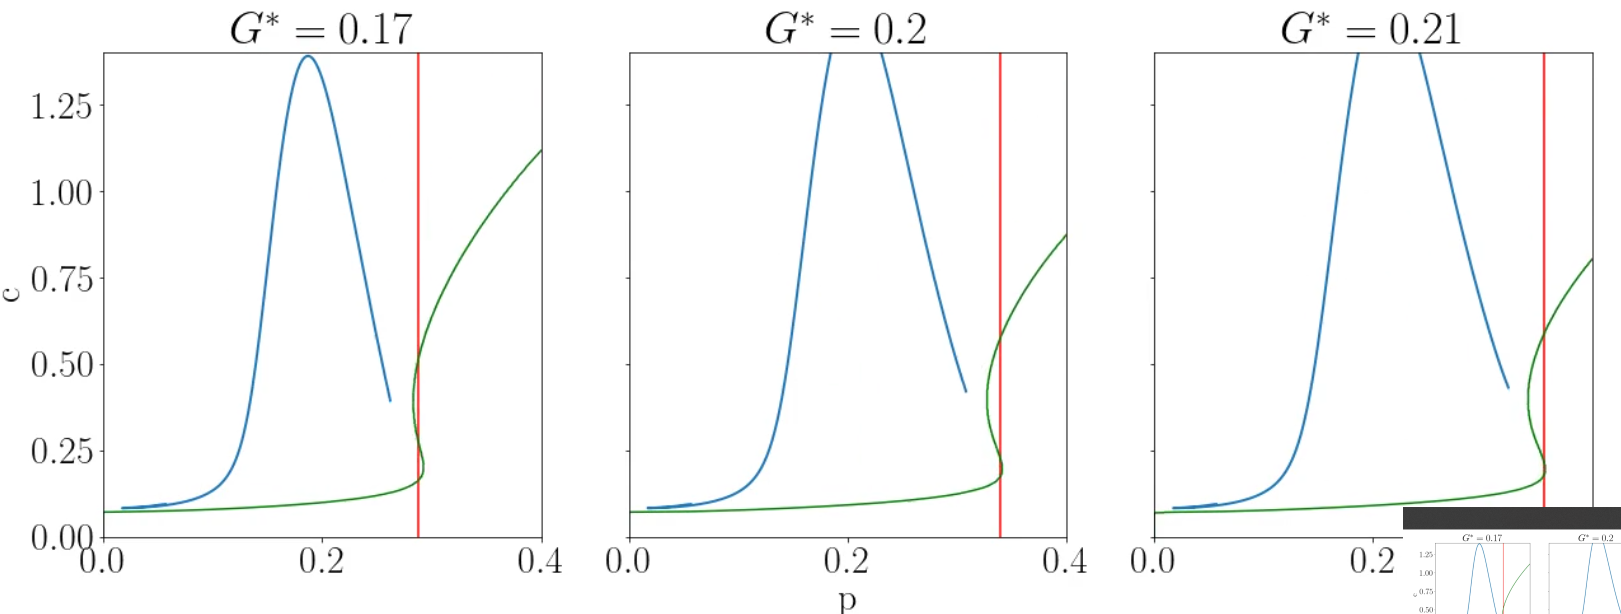
\includegraphics[width=0.7\linewidth]{snapshot_of_trajectory_animation_no_feedback.png}
	\centering
	\caption{Screenshot of trajectories of system depicting delays in reaching stable limit cycle. The movie is titled ``feedback\_off\_nc\_trajectory.mp4''. The green line depicts the calcium nullcline, and the red line depicts the IP3 nullcline.}
	\label{fig:oscillation_animation}
\end{figure} 

We have not found evidence of a saddle node bifurcation in the parameter region that might explain the delay. Qualitatively watching the movie, it seems like the trajectory "comes close" to a sort of steady state near the intersection of calcium and IP3 nullclines. Later, we might try to explore this quantitatively by seeing how close the trajectory gets to the unstable fixed point inside of the limit cycle.

I also plan to examine starting the system at different initial values. Looking at Fig \ref{fig:v3k_2_gstar_steps}, it seems as though stepping up to higher values of $G^*$ incurs more of a delay than stepping down to lower ones. It may be that the region of delay is avoided by starting with different values of $c_{tot}$ or $h$.

For now, this section is inconclusive.





%%%%%%%%%%%%%%%%%%%%%%%%%%%%%%%%%%%%%%%

%%%%%%%%%%%%%%%%%%%%%%%%%%%%%%%%%%%%%%%





\section{Glutamate GPCR Model}

To complete the dynamical system, we add the glutamate GPCR dynamics to the system, including the dynamics for $G^*$ which is an input to the remaining IP3/calcium system. The new equations to be added are

\begin{align}
\frac{dG^*}{dt} &= k_+ \phi G - k_- G^* - k_{d1} G^* \\
\frac{dG_{d1}}{dt} &= k_{d1}G^* - k_{r1} G_{d1} \\
\frac{dG_{d2}}{dt} &= k_{d2}G^* G - k_{r2} G_{d2}
\end{align}
where $G$ is given implicitly as $G = 1 - G^* - G_{d1} - G_{d2}$ and $\phi$ represent the concentration of glutamate in micromolar. A bifurcation for the new system with calcium as the variable and glutamate as the control parameter is given in Fig \ref{fig:c_glut_bifurcation}. Notably in this plot, the system is highly sensitive to glutamate, as oscillations begin for fairly small values of $\phi$. In Fig \ref{fig:c_glut_bifurcation_pos_neg}, we see that positive IP3 to calcium feedback seems to drive the left Hopf bifurcation closer to $\phi=0$, so we may want to adjust this. We can also consider modifying the glutamate sensitivity of the system by changing the $k_+$ parameter.

\begin{figure}[H]
	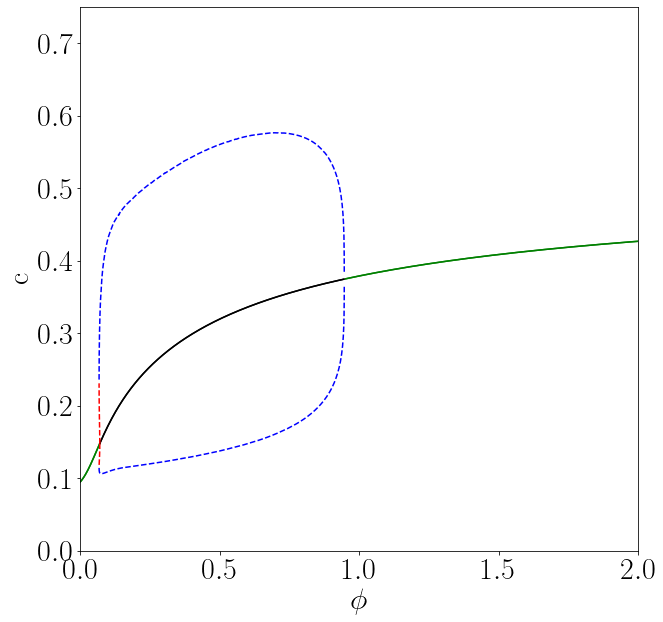
\includegraphics[width=0.6\linewidth]{c_glut_bifurcation.png}
	\centering
	\caption{Bifurcation plot for full GPCR, IP3, calcium system, showing calcium as the variable and glutamate as the control parameter.}
	\label{fig:c_glut_bifurcation}
\end{figure}

\begin{figure}[H]
	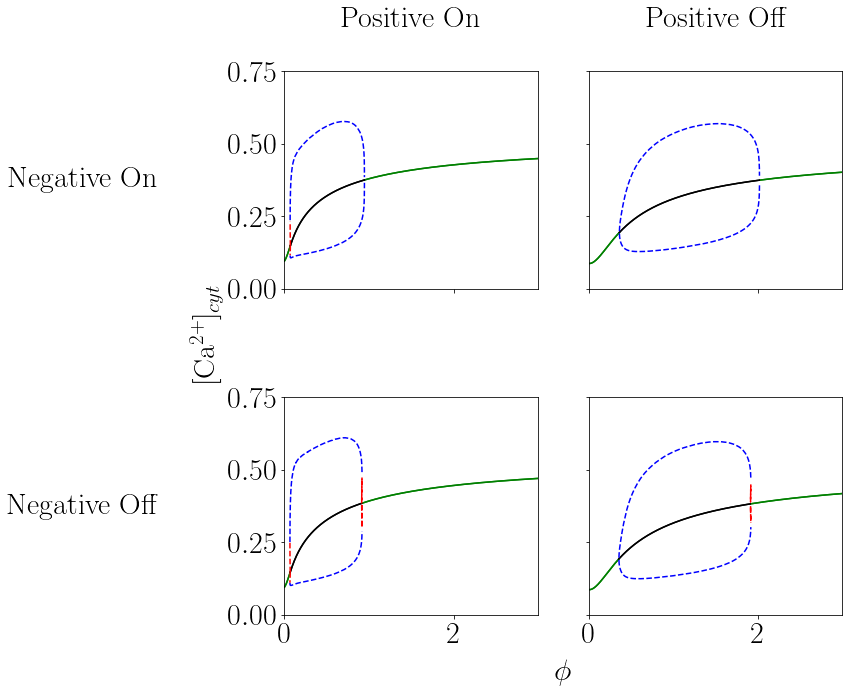
\includegraphics[width=0.6\linewidth]{gpcr_positive_negative_bifurcations.png}
	\centering
	\caption{Bifurcation plot for full GPCR, IP3, calcium system, with IP3 to calcium feedback turned on or off.}
	\label{fig:c_glut_bifurcation_pos_neg}
\end{figure}

\subsection{Heterologous Deactivation (Gd2)}

One novel addition to the GPCR model is a heterlogous deactivation variable, in which $G$ can be deactivated more slowly, but have deactivation last for a longer period of time. Currently we are modeling this as requiring both $G$ and $G^*$, calling it heterologous deactivation $G_{d2}$. However, currently it is effectively non-existent, as $G_{d2}$ never becomes appreciably large, as can be seen in Fig \ref{fig:GPCR_bath_variables_range_glut} (noting that we are mostly considering glutamate concentrations around $0$ to $0.4$). Alla has suggested that perhaps the generation of $G_{d2}$ needs to be dependent on a variable that is further downstream and decoupled from the dynamics of the GPCR, or we might need to add some other decoupled variable to the system to give $G_{d2}$ the properties that we want it to have.

\begin{figure}[H]
	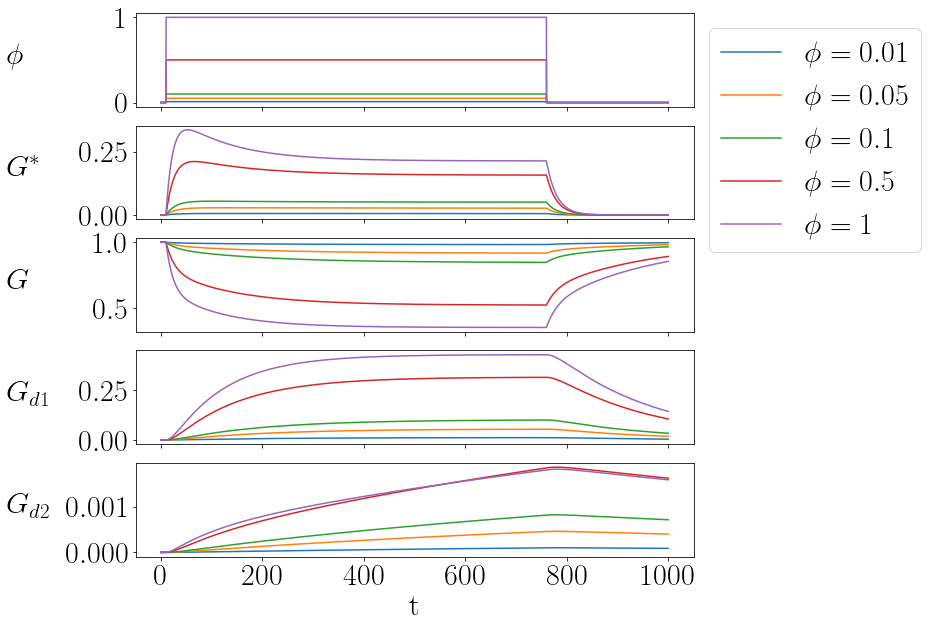
\includegraphics[width=0.7\linewidth]{Gd2_long_equilibria_bath_01_1.png}
	\centering
	\caption{Solutions to all variables of the glutamate GPCR system when given a range of glutamate bath strengths ranging from $0.01$ to $1$.}
	\label{fig:GPCR_bath_variables_range_glut}

\end{figure}

\subsection{Classifying Calcium Response}

In Section 1.2, we mentioned that Marsa identified four types of calcium response. Using the new system including IP3 and the GPCR dynamics, we would like to see if we can reproduce these four calcium responses for a range of glutamate inputs. First, I reproduced the calcium response classification code in Python, and the results of attempting to reproduce Figure 4 from \cite{taheri2017diversity} are shown in Fig \ref{fig:ip3_classification}. Notably, not all of the responses are classified in the same way as the original paper. I intend to dig into individual cases to see where they differ, as well as attempt to reproduce other figures detailing frequency of responses with specific ranges of double exponential input parameters.

\begin{figure}[H]
	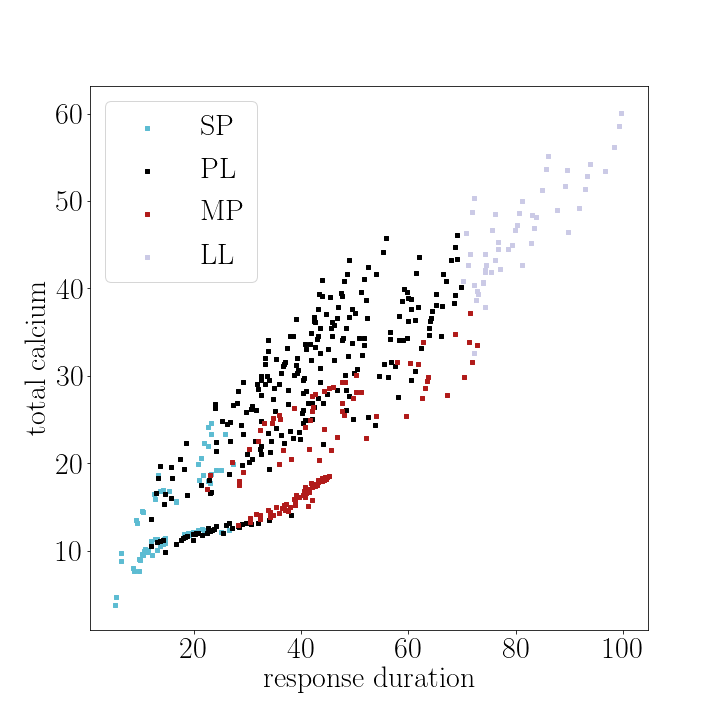
\includegraphics[width=0.6\linewidth]{ip3_classification.png}
	\centering
	\caption{Reproduction of Figure 4 from \cite{taheri2017diversity} using rewritten Python code. }
	\label{fig:ip3_classification}
\end{figure}

\begin{figure}[H]
	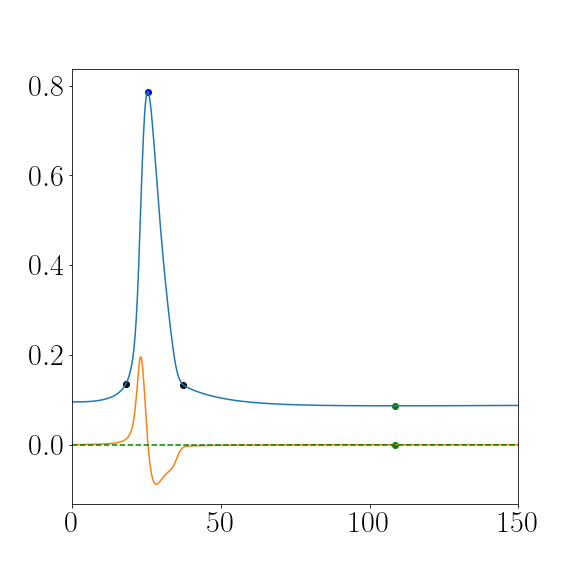
\includegraphics[width=0.3\linewidth]{SP_example.png}
	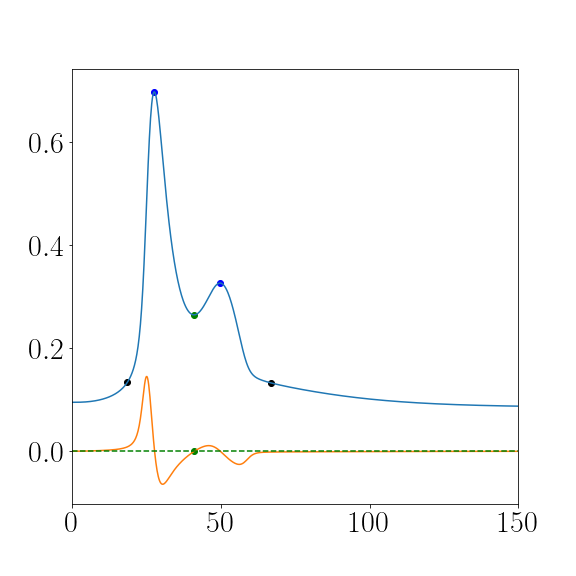
\includegraphics[width=0.3\linewidth]{MP_example.png}
	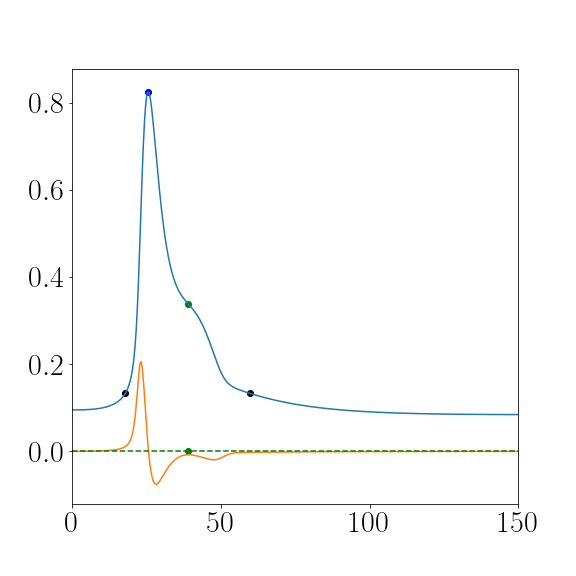
\includegraphics[width=0.3\linewidth]{PL_example.png}
	\centering
	\caption{Examples of calcium responses with the full dynamical system. Blue shows the calcium response, while orange shows the derivative of calcium. Scatter points label where algorithm divides different peak responses.}
	\label{fig:glut_classification_examples}
\end{figure}

In Fig \ref{fig:glut_classification_examples} we show examples of some of the responses we are able to elicit with the system. One of the main issues currently is that the troughs between peaks are not deep enough to be considered a MP response by the current algorithm. This may be due to the delays in oscillation caused by negative IP3 to calcium feedback making it difficult for the system to reach an oscillatory regime that will show up as multiple peaks. We must further decide how much negative feedback we are indeed willing to accept for this system. Nevertheless, we create the same scatter plot as Fig \ref{fig:ip3_classification} with the whole system in Fig \ref{fig:glut_classification}.

\begin{figure}[H]
	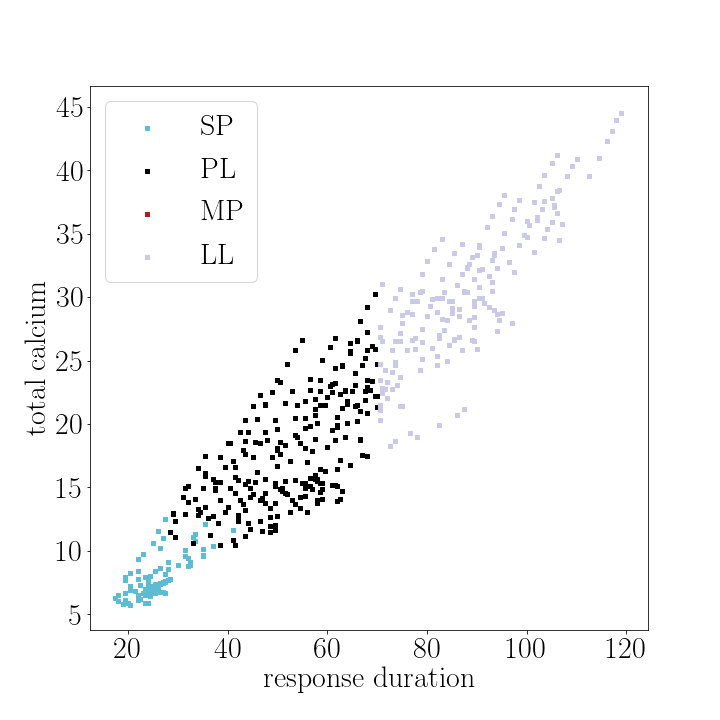
\includegraphics[width=0.7\linewidth]{glut_classification.png}
	\centering
	\caption{Classification of responses for a range of glutamate double exponential curves, arranged by total length of response and total calcium produced during the response. }
	\label{fig:glut_classification}
\end{figure}

\pagebreak

\bibliography{references}
\bibliographystyle{ieeetr}

\end{document}